\subsubsection{The solitary wave benchmark}
\label{sec:benchmark-solitary_wave}

\textit{This section was contributed by Juliane Dannberg and is based on a section in \cite{dannberg_melt} by Juliane Dannberg and Timo Heister.}

One of the most widely used benchmarks for codes that model the migration of melt through a compacting and dilating matrix is the propagation of solitary waves (e.g. \cite{SS11, KMK2013, Schm00}).
The benchmark is intended to test the accuracy of the solution of the two-phase flow equations as described in Section \ref{sec:melt_transport} and makes use of the fact that there is an analytical solution for the shape of solitary waves that travel through a partially molten rock with a constant background porosity without changing their shape and with a constant wave speed.
Here, we follow the setup of the benchmark as it is described in \cite{BR86}, which considers one-dimensional solitary waves.

The model features a perturbation of higher porosity with the amplitude $A \phi_0$ in a uniform low-porosity ($\phi=\phi_0$) background.  Due to its lower density, melt migrates upwards, dilating the solid matrix at its front and compacting it at its end.

Assuming constant shear and compaction viscosities and using a permeability law of the form
%
\begin{align*}
k_\phi &= k_0 \phi^3, && \text{ implying a Darcy coefficient }
K_D(\phi) = \frac{k_0}{\eta_f} \phi^3 , \\
\intertext{and the non-dimensionalization }
x &= \delta x'
  && \text{ with the compaction length } \delta = \sqrt{K_D(\phi_0)(\xi + \frac{4}{3}\eta)} , \\
\phi &= \phi_0 \phi '
  && \text{ with the background porosity } \phi_0 , \\
(\mathbf u_s, \mathbf u_f) &= u_0 (\mathbf u_s, \mathbf u_f)'
  && \text{ with the separation flux } \phi_0 u_0 = K_D(\phi_0) \Delta\rho g ,
\end{align*}
%
the analytical solution for the shape of the solitary wave can be written in implicit form as:
\begin{align*}
x(\phi) &= \pm (A + 0.5)
\left[ -2 \sqrt{A-\phi} + \frac{1}{\sqrt{A-1}}
\ln \frac{\sqrt{A-1} - \sqrt{A-\phi}}{\sqrt{A-1} + \sqrt{A-\phi}} \right]
\end{align*}
and the phase speed $c$, scaled back to physical units, is $c = u_0 (2A+1)$.
This is only valid in the limit of small porosity $\phi_0 \ll 1$. Figure~\ref{fig:setup-solitary-wave} illustrates the model setup.

\begin{figure}
  \begin{center}
    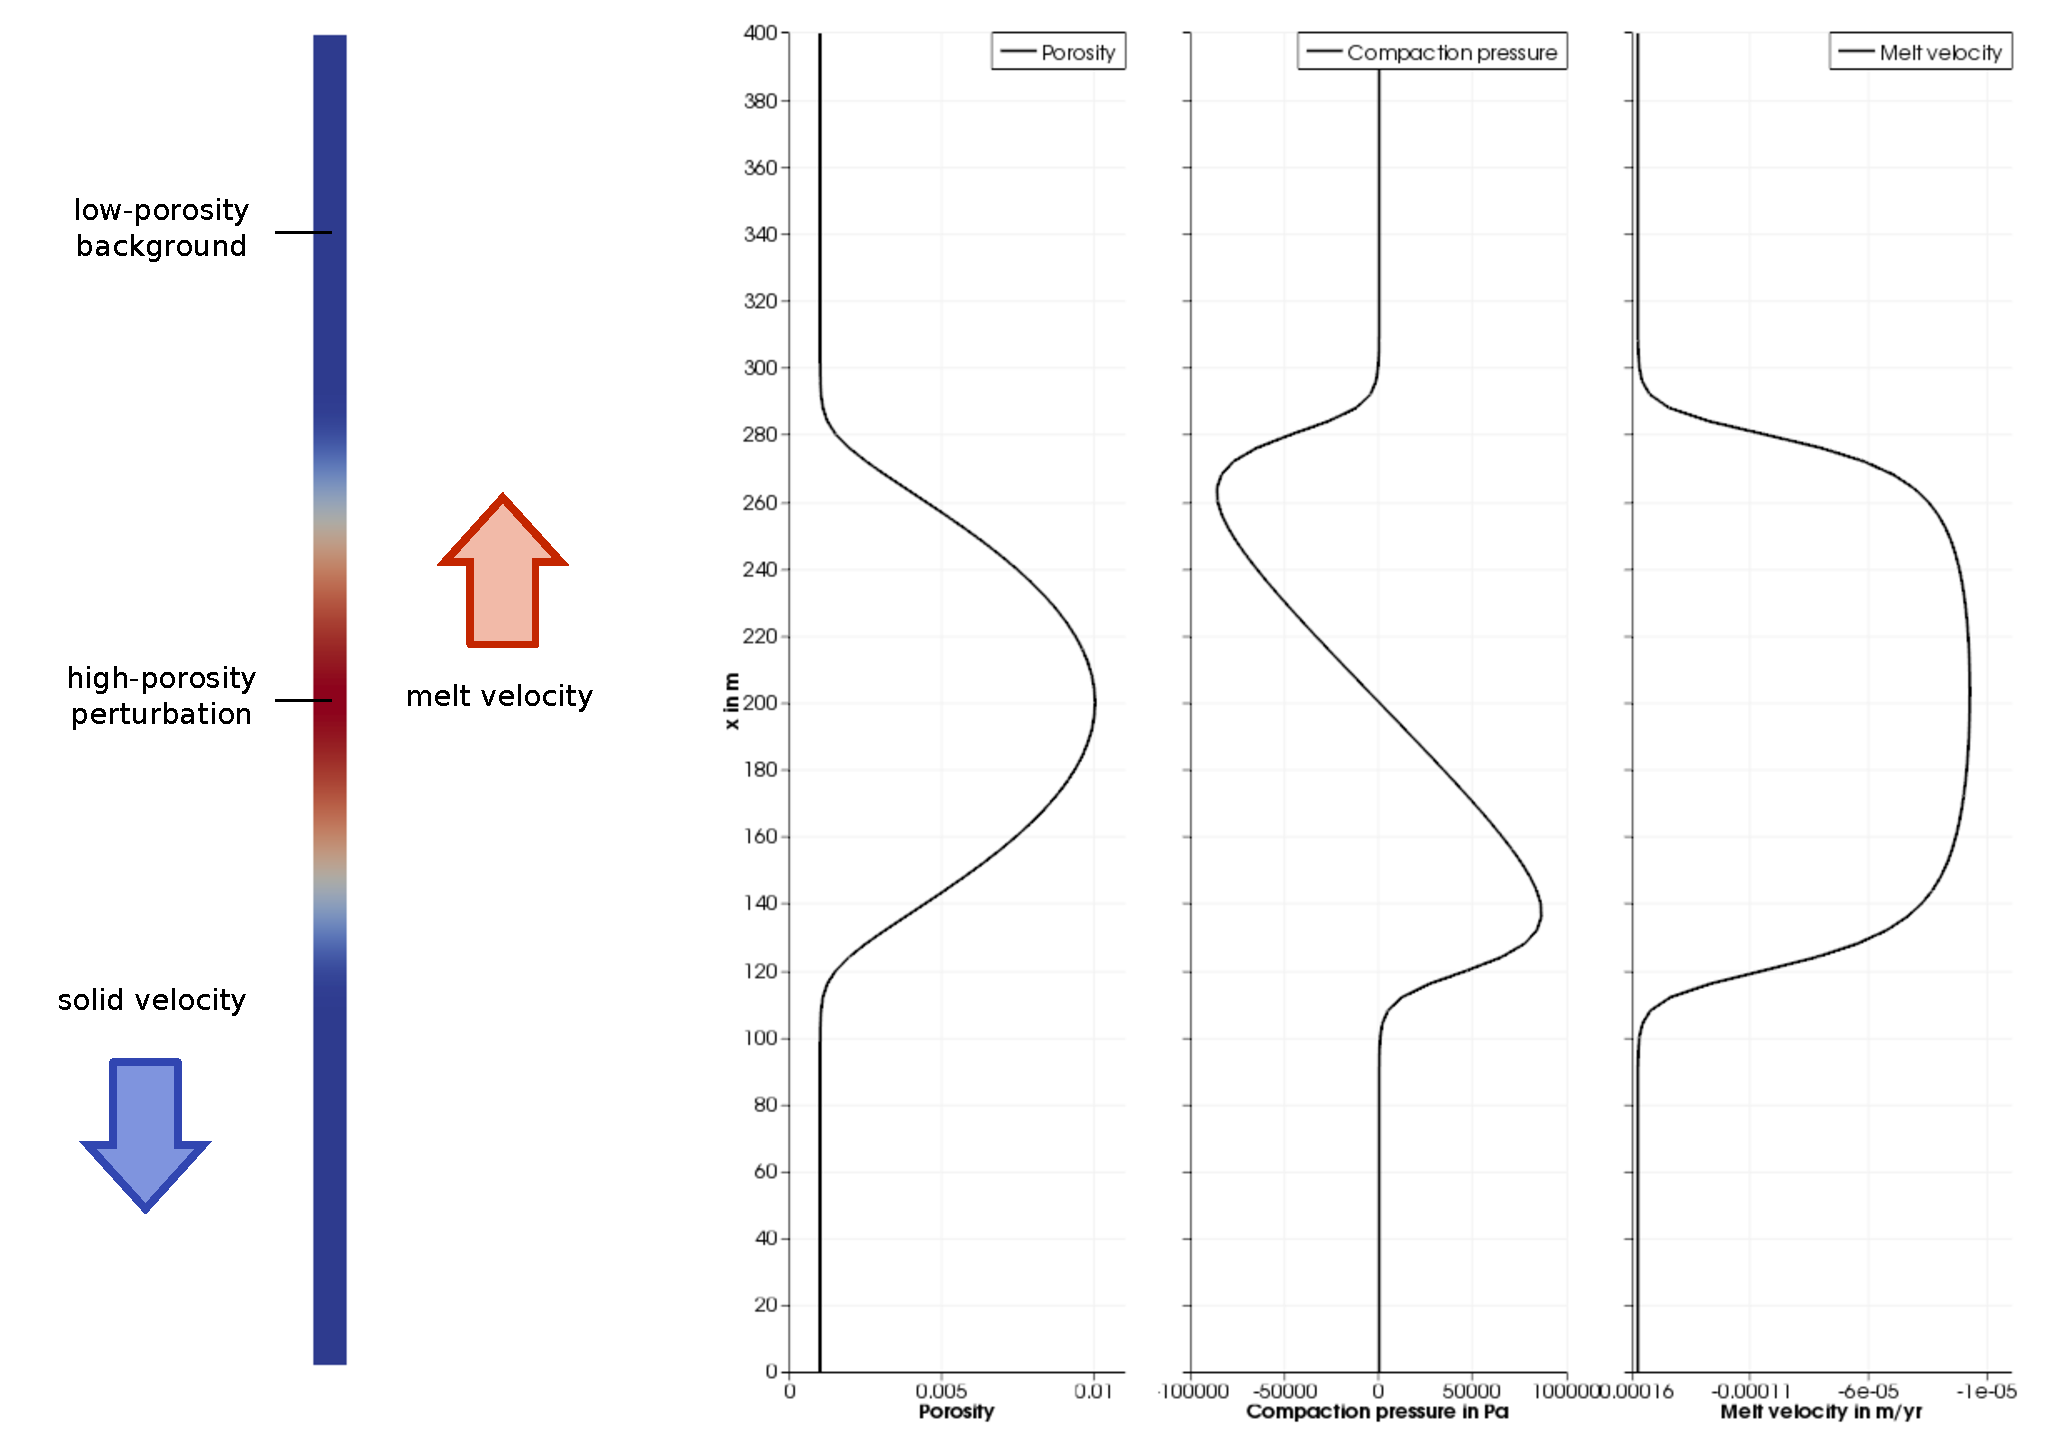
\includegraphics[width=0.65\textwidth]{cookbooks/benchmarks/solitary_wave/doc/setup.pdf}
  \end{center}
  \caption{\it Setup of the solitary wave benchmark. The domain is $400$ m high and includes a low porosity
  ($\phi = 0.001$) background with an initial perturbation ($\phi = 0.1$). The solid density is $3300\,kg/m^3$
  and the melt density is $2500\,kg/m^3$. We apply the negative phase speed
  of the solitary wave $\mathbf u_s = -c \, \mathbf e_z$ as velocity boundary condition, so that the wave will
  stay at its original position while the background is moving.}
  \label{fig:setup-solitary-wave}
\end{figure}

The parameter file and material model for this setup can be found in \url{benchmarks/solitary_wave/solitary_wave.prm} and \url{benchmarks/solitary_wave/solitary_wave.cc}. The most relevant sections are shown in the following paragraph.

\lstinputlisting[language=prmfile]{cookbooks/benchmarks/solitary_wave/doc/solitary_wave.prm.out}

The benchmark uses a custom model to generate the initial condition for the porosity field as specified by the analytical solution, and its own material model, which includes the additional material properties needed by models with melt migration, such as the permeability, melt density and compaction viscosity. The solitary wave postprocessor compares the porosity and pressure in the model to the analytical solution, and computes the errors for the shape of the porosity, shape of the compaction pressure and the phase speed.
We apply the negative phase speed of the solitary wave as a boundary condition for the solid velocity. This changes the reference frame, so that the solitary wave stays in the center of the domain, while the solid moves downwards. The temperature evolution does not play a role in this benchmark, so all temperature and heating-related parameters are disabled or set to zero.

And extensive discussion of the results and convergence behavior can be found in \cite{dannberg_melt}.
